%
% main.tex -- Paper zum Thema <clifford>
%
% (c) 2020 Hochschule Rapperswil
%
\chapter{Clifford Algebra\label{chapter:clifford}}
\lhead{Clifford Algebra}
\begin{refsection}
\chapterauthor{Thierry Schwaller, Marius Baumann}



Der Nutzen, welche die Clifford Algebra hat, lässt sich am besten mit den Worten des modernen Begründers dieser erläutern.

"GA [Geometric Algebra i.a.W. Clifford Algebra] provides a unified language for the whole of physics and for much of mathematics and its applications that is conceptually and computationally superior to alternative mathematical systems in many application domains." \cite{clifford:hestenes_GA} 

Im folgenden hoffen wir den Leser von der Nützlichkeit und der geometrischen Schönheit der Clifford Algebra zu überzeugen.
\section{Vektoroperationen\label{clifford:section:Vektoroperationen}}
\rhead{Vektoroperationen}
\subsection{Vektordarstellung\label{clifford:section:Vektordarstellung}}
Vektoren können neben der üblichen Darstellung, auch als Linearkombination aus Basisvektoren dargestellt werden
\begin{equation}
    \begin{split}
    \textbf{a} 
    &=
    \begin{pmatrix} 
    a_1 \\ a_2 \\ \vdots \\ a_n   
    \end{pmatrix} 
    =
    a_1 \begin{pmatrix}
    1 \\ 0 \\ \vdots \\ 0  
    \end{pmatrix} 
    + 
    a_2\begin{pmatrix} 
    0 \\ 1 \\ \vdots \\ 0  
    \end{pmatrix} + \dots 
    + 
    a_n\begin{pmatrix}
    0 \\ 0 \\ \vdots \\ 1  
    \end{pmatrix} \\\ 
    &= 
    a_1\textbf{e}_1 
    +
    a_2\textbf{e}_2
    + 
    \dots + a_n\textbf{e}_n
    = 
    \sum_{i=1}^{n} a_i \textbf{e}_i
    \qquad
    a_i \in \mathbb{R}
    , \textbf{e}_i \in \mathbb{R}^n.
    \end{split}
\end{equation}
Diese Basisvektoren sollen orthonormal sein und um die Darstellung zu vereinfachen werden sie durch $\textbf{e}_1 , \textbf{e}_2, ...$ ersetzt.
\begin{beispiel}
Linearkombination von Basisvektoren in $\mathbb{R}^4$
    \begin{equation}
        \begin{pmatrix} 
        42 \\ 2 \\ 1291 \\ 4    
        \end{pmatrix} 
        = 
        42 \begin{pmatrix}
        1 \\ 0 \\ 0 \\ 0 
        \end{pmatrix} 
        +
        2 \begin{pmatrix} 
        0 \\ 1 \\ 0 \\ 0 
        \end{pmatrix}
        +
        1291 
        \begin{pmatrix} 
        0 \\ 0 \\ 1 \\ 0 
        \end{pmatrix} 
        +
        4 \begin{pmatrix} 
        0 \\ 0 \\ 0 \\ 1 
        \end{pmatrix} 
        = 
        42\textbf{e}_1
        + 
        2\textbf{e}_2
        + 
        1291\textbf{e}_3
        + 
        4\textbf{e}_4
    \end{equation}
\end{beispiel}
Wobei Beispiel für einen vier dimensionalen Vektor ist, dies kann selbstverständlich für beliebig viele Dimensionen nach demselben Schema erweitert werden.
\subsection{Quadrat von Vektoren}
Was eine Addition von Vektoren bedeutet ist sehr intuitiv und auch leicht geometrisch darzustellen, was allerdings das Produkt von Vektoren ergibt mag anfänglich unintuitiv wirken. 
Was soll es schon heissen zwei Vektoren miteinander zu multiplizieren? 
\newline
Im Folgenden werden wir versuchen diese Operation ähnlich intuitiv darzustellen.
\newline
Um sinnvoll eine neue Operation zwischen zwei Elementen einer Algebra, in diesem Fall Vektoren, zu definieren, muss man überlegen, was das Ziel dieser Operation ist. 
Als grundsätzliches Ziel wird definiert, dass das Quadrat eines Vektor dessen Länge im Quadrat ergibt, da dies auch in vielen anderen Bereichen der Mathematik,zum Beispiel bei komplexen Zahlen, auch so definiert ist.  
\newline 
Zusätzlich wollen wir auch das Assoziativgesetz und das Kommutativgesetz für Skalare beibehalten. Wobei das Kommutativgesetz leider, oder wie man sehen wird zum Glück, in der geometrischen Algebra im generellen nicht mehr gilt. Das heisst wir dürfen ausklammern \ref{eq:assoziativ} und die Position von Skalaren im Produkt ändern \ref{eq:kommSkalar}, allerdings nicht die Position der Vektoren \ref{eq:kommVector}.
\begin{equation}
    \label{eq:assoziativ}
    \textbf{e}_i(\textbf{e}_j + \textbf{e}_k) 
    = 
    \textbf{e}_i\textbf{e}_j + \textbf{e}_i\textbf{e}_k 
\end{equation}
\begin{equation}
    \label{eq:kommSkalar}
    a\textbf{e}_ib\textbf{e}_j 
    = 
    ab\textbf{e}_i\textbf{e}_j
\end{equation}
\begin{equation}
    \label{eq:kommVector}
    \textbf{e}_i\textbf{e}_j 
    \neq 
    \textbf{e}_j\textbf{e}_i
\end{equation}
Betrachten wir nun mit diesen Regeln das Quadrat eines Vektors.
\begin{align}
    \textbf{a}^2 &= 
    \left ( 
    \sum_{i=1}^{n} a_i \textbf{e}_i 
    \right ) 
    \left ( 
    \sum_{i=1}^{n} a_i \textbf{e}_i 
    \right )
    \label{eq:quad_a_1}
    \\
    &= 
    \textcolor{red}{\sum_{i=1}^{n} a_i^2\textbf{e}_i^2} 
    + 
    \textcolor{blue}{\sum_{\begin{subarray}{l}i,j=1\\i \neq j\end{subarray}}^n  a_ia_j\textbf{e}_i\textbf{e}_j } 
    \label{eq:quad_a_2}
    \\
    &= \textcolor{cyan}{\sum_{i=1}^{n} a_i^2} + \textcolor{orange}{\sum_{\begin{subarray}{l}i,j=1\\i \neq j\end{subarray}}^n  a_ia_j\textbf{e}_i\textbf{e}_j}.
    \label{eq:quad_a_3}
\end{align}

\begin{beispiel}
Quadrat eines Vektors in $\mathbb{R}^2$
\begin{equation}
    \begin{split}
    \textbf{a}^2 
    &= (a_1\textbf{e}_1+a_2\textbf{e}_2)(a_1\textbf{e}_1+a_2\textbf{e}_2) \\\
    &= \textcolor{red}{a_1^2\textbf{e}_1^2 + a_2^2\textbf{e}_2^2} 
    + \textcolor{blue}{a_1\textbf{e}_1a_2\textbf{e}_2 + a_2\textbf{e}_2a_1\textbf{e}_2}   \\\
    & = \textcolor{cyan}{a_1^2 + a_2^2} + \textcolor{orange}{a_1b\textbf{e}_1a_2\textbf{e}_2 + a_2\textbf{e}_2a_1\textbf{e}_2}
    \end{split}
\end{equation}

\end{beispiel}
Der Vektor wird in \ref{eq:quad_a_1} als Linearkombination geschrieben.
Das Quadrat kann, wie in \ref{eq:quad_a_2} gezeigt, in zwei Summen aufteilen werden , wobei die roten Summe die quadrierten Terme und die blaue Summe die Mischterme beinhaltet. 
\newline
Da $\textbf{e}_i^2 = 1$ gilt, da zuvor vorausgesetzt wurde, dass man mit orthonormalen Einheitsvektoren arbeitet, wird dies nun eingesetzt ergibt sich \ref{eq:quad_a_3}
\newline
Die hellblaue Teil ist nun bereits Länge im Quadrat eines Vektors, also das Ziel der Multiplikation. 
Daher muss der restliche Teil dieser Gleichung null ergeben. 
Aus dieser Erkenntnis leiten wir in \ref{eq:Mischterme_Null} weitere Eigenschaften für die Multiplikation her.
\begin{equation}
    \label{eq:Mischterme_Null}
    \sum_{\begin{subarray}{l}i,j=1\\i \neq j\end{subarray}}^n  a_ia_j\textbf{e}_i\textbf{e}_j  = \textcolor{blue}{a_1a_2(\textbf{e}_1\textbf{e}_2 + \textbf{e}_2\textbf{e}_1)} + a_1a_3(\textbf{e}_1\textbf{e}_3 + \textbf{e}_3\textbf{e}_1) + \dots =  0
\end{equation}
Da dies für beliebige $a_i$ gelten muss werden alle Terme bis auf $a_1$ und $a_2$ gleich null gesetzt. Somit fallen alle Terme bis auf den blauen weg. Wird dies weiter vereinfacht ergibt sich
\begin{equation}
\begin{split}
    a_1a_2(\textbf{e}_1\textbf{e}_2 + \textbf{e}_2\textbf{e}_1) &= 0 \\
    a_1a_2\textbf{e}_1\textbf{e}_2 &= -a_1a_2\textbf{e}_2\textbf{e}_1 \\
    \textbf{e}_1\textbf{e}_2 &= -\textbf{e}_2\textbf{e}_1.
\end{split}
\end{equation}
\begin{satz}
    Die Multiplikation von Vektoren ist antikommutativ, wenn die multiplizierten Vektoren orthogonal sind.
    \begin{equation}
        \textbf{e}_i\textbf{e}_j = -\textbf{e}_j\textbf{e}_i \qquad \textbf{e}_i \perp \textbf{e}_j
    \end{equation}
\end{satz}
Dieses Wissen reicht nun bereits um alle Produkte der Basisvektoren zu berechnen, was in \ref{tab:multip_vec} gemacht wurde.
\begin{table}
\caption{Multiplikationstabelle für Vektoren}
\label{tab:multip_vec}
\begin{center}
\begin{tabular}{ |c|c|c|c|c|c| } 
 \hline
  & $\textbf{e}_1$ & $\textbf{e}_2$ & $\dots$ & $\textbf{e}_{n-1}$ & $\textbf{e}_{n}$ \\
  \hline
 $\textbf{e}_1$ & 1 & $\textbf{e}_1\textbf{e}_2$ & $\dots$ & $\textbf{e}_1\textbf{e}_{n-1}$ & $\textbf{e}_1\textbf{e}_{n}$ \\
 \hline
 $\textbf{e}_2$ & $-\textbf{e}_1\textbf{e}_2$ & 1 & $\dots$ & $\textbf{e}_2\textbf{e}_{n-1}$ & $\textbf{e}_2\textbf{e}_{n}$ \\
 \hline
 $\vdots$ & $\vdots$ & $\vdots$ & $\ddots$ & $\vdots$ & $\vdots$ \\
 \hline
 $\textbf{e}_{n-1}$ & $-\textbf{e}_1\textbf{e}_{n-1}$ & $-\textbf{e}_2\textbf{e}_{n-1}$  & $\dots$ & $1$ & $\textbf{e}_{n-1}\textbf{e}_{n}$ \\
 \hline
 $\textbf{e}_{n}$ & $-\textbf{e}_1\textbf{e}_{n}$ & $-\textbf{e}_2\textbf{e}_{n}$  & $\dots$ & $-\textbf{e}_{n-1}\textbf{e}_{n}$ & 1 \\
 \hline
\end{tabular}
\end{center}
\end{table}
\subsection{Multiplikation von Vektoren}
Was geschieht nun wenn zwei beliebige Vektoren,$u$ und $v$, miteinander multipliziert werden?
\begin{equation}
    \textbf{u} = 
    \sum_{i=1}^{n} u_i \textbf{e}_i 
    \qquad 
    \textbf{v} = \sum_{i=1}^{n} v_i \textbf{e}_i
\end{equation}
\begin{equation}
    \begin{split}
        \textbf{u}\textbf{v} 
        =
        \left ( 
        \sum_{i=1}^{n} u_i \textbf{e}_i
        \right ) 
        \left ( 
        \sum_{i=1}^{n} v_i \textbf{e}_i
        \right) 
        = 
        \sum_{i=1}^n u_iv_i\underbrace{\textbf{e}_i^2}_{1} 
        + \sum_{\begin{subarray}{l}i,j=1\\i \neq j\end{subarray}}^n  u_iv_j\textbf{e}_i\textbf{e}_j 
    \end{split}
\end{equation}
\begin{beispiel}
    Multiplikation von Vektoren in $\mathbb{R}^2$
\end{beispiel}
\begin{equation}
    \begin{split}
        \textbf{u}\textbf{v} 
        &= 
        (u_1\textbf{e}_1 + u_2\textbf{e}_2)(v_1\textbf{e}_1 + v_2\textbf{e}_2) 
        = 
        u_1v_1\textbf{e}_1^2
        + 
        u_2v_2\textbf{e}_2^2 
        + 
        u_1v_2\textbf{e}_1\textbf{e}_2 
        +  
        u_2v_1\underbrace{\textbf{e}_2\textbf{e}_1}_{-\textbf{e}_1\textbf{e}_2}
        \\\ 
        &=  
        \underbrace{(u_1v_1 + u_2v_2)}_{\text{Skalarprodukt}} 
        + 
        \underbrace{(u_1v_2 - u_2v_1)\textbf{e}_1\textbf{e}_2}_{\text{Äusseres Produkt}}
    \end{split}
\end{equation}
Der linke Teil dieser Multiplikation ergibt das Skalarprodukt der zwei Vektoren, der rechte Term ergibt etwas neues das sich das äussere Produkt der zwei Vektoren nennt.
\subsubsection{Äusseres Produkt}
Das äussere Produkt von zwei Vektoren wird mit einem $\wedge$ dargestellt
\begin{equation}
    \textbf{u}\wedge \textbf{v} 
    = 
    \sum_{\begin{subarray}{l}i,j=1\\i \neq j\end{subarray}}^n  u_iv_j\textbf{e}_i\textbf{e}_j 
\end{equation}
\begin{beispiel}
Äusseres Produkt von zwei Vektoren in $\mathbb{R}^3$
\end{beispiel}
\begin{equation}
    \begin{split}
        u \wedge v 
        &= 
        u_1v_2\textbf{e}_1\textbf{e}_2 
        + 
        u_1v_3\textbf{e}_1\textbf{e}_3 
        + 
        u_2v_2\textbf{e}_2\textbf{e}_3 
        + 
        u_2v_1\textbf{e}_2\textbf{e}_1 
        + 
        u_3v_1\textbf{e}_3\textbf{e}_1 
        +
        u_3v_2\textbf{e}_3\textbf{e}_2 \\\ 
        &= 
        (u_1v_2 - u_2v_1)\textbf{e}_1\textbf{e}_2 
        + 
        (u_1v_3 - v_3u_1)\textbf{e}_1\textbf{e}_3 
        + 
        (u_2v_3 - u_3v_2)\textbf{e}_2\textbf{e}_3
    \end{split}
\end{equation}
Im letzten Schritt des Beispiels wurden nun, mit Hilfe der antikommutativität des Produkts, die Vektorprodukte, welche die gleichen Einheitsvektoren beinhalten, zusammengefasst. Dieses Vorgehen kann man auch allgemein anwenden, wie in den Gleichungen \ref{eq:u_wedge_v}-\ref{eq:u_wedge_v_5} hergeleitet.
\begin{align}
        \textbf{u}\wedge \textbf{v}
        &= 
        \sum_{\begin{subarray}{l}i,j=1\\i \neq j\end{subarray}}^n  
        u_iv_j\textbf{e}_i\textbf{e}_j 
        \label{eq:u_wedge_v}
        \\
        \label{eq:u_wedge_v_1}
        &= 
        \sum_{\begin{subarray}{l}i,j=1\\i < j\end{subarray}}^n u_iv_j\textbf{e}_i\textbf{e}_j 
        + 
        \sum_{\begin{subarray}{l}i,j=1\\j < i\end{subarray}}^n u_iv_j\textbf{e}_i\textbf{e}_j 
        \\
        \label{eq:u_wedge_v_2}
        &= 
        \sum_{\begin{subarray}{l}i,j=1\\i < j\end{subarray}}^n u_iv_j\textbf{e}_i\textbf{e}_j 
        + 
        \sum_{\begin{subarray}{l}i,j=1\\i < j\end{subarray}}^n u_jv_i\textbf{e}_j\textbf{e}_i
        \\
        \label{eq:u_wedge_v_3}
        &= 
        \sum_{\begin{subarray}{l}i,j=1\\i < j\end{subarray}}^n u_iv_j\textbf{e}_i\textbf{e}_j 
        - 
        \sum_{\begin{subarray}{l}i,j=1\\i < j\end{subarray}}^n u_jv_i\textbf{e}_i\textbf{e}_j
        \\
        \label{eq:u_wedge_v_4}
        &= 
        \sum_{\begin{subarray}{l}i,j=1\\i < j\end{subarray}}^n (u_iv_j -u_jv_i)\textbf{e}_i\textbf{e}_j
        \\
        \label{eq:u_wedge_v_5}
        &= 
        \sum_{\begin{subarray}{l}i,j=1\\i < j\end{subarray}}^n \begin{vmatrix} 
        u_i & v_i \\
        u_j & v_j
    \end{vmatrix}\textbf{e}_i\textbf{e}_j
\end{align}
Die Summe aus \ref{eq:u_wedge_v_1} wird in \ref{eq:u_wedge_v} in zwei verschiedene Summen aufgeteilt. 
Wobei die linke Summe jeweils den Basisvektor mit dem höheren Index an erster Stelle und die rechte Summe diesen jeweils an zweiter Stelle hat. 
\newline
Bei \ref{eq:u_wedge_v_2} werden die Indexe der zweiten Summe vertauscht, damit man nun bei beiden Teilen die gleiche Summe hat.
Danach werden in \ref{eq:u_wedge_v_3}, mit Hilfe der Antikommutativität, die Einheitsvektoren der zweiten Summe vertauscht.
\newline
Nun können die Summen, wie in \ref{eq:u_wedge_v_4} wieder in eine Summe zusammengefasst werden.
\newline
Der Term in der Klammer in \ref{eq:u_wedge_v_4} kann auch als Determinante einer 2x2 Matrix dargestellt werden, was in \ref{eq:u_wedge_v_5} gemacht wird.
\newline
Die Determinante einer Matrix beschreibt welche von den Spaltenvektoren aufgespannt wird, wie in Abbildung \ref{figure:det} dargestellt.
\begin{figure}
\centering
\begin{tikzpicture}
  \draw[thin,gray!40] (0,0) grid (4,4);
  \draw[<->] (0,0)--(4,0) ;
  \draw[<->] (0,0)--(0,4) ;
  \draw[line width=0,fill=gray!40] (0,0)--(3,1)--(4,3)--(1,2);
  \draw[line width=2pt,blue,-stealth](0,0)--(3,1) node[anchor=north
  west]{$\boldsymbol{u}$};
  \draw[line width=2pt,red,-stealth](0,0)--(1,2) node[anchor=south east]{$\boldsymbol{v}$};
  \draw[black] (2,1.5)--(-0.5,2.5) node[anchor = east]{$\begin{vmatrix} 
        u_i & v_i \\
        u_j & v_j
    \end{vmatrix} = u_iv_j - v_iu_j$};
\end{tikzpicture}
\caption{Geometrische Interpretation der Determinante einer 2x2 Matrix\label{figure:det}}
\end{figure}
\newline
Das äussere Produkt besteht nun also aus der Summe 
    $\sum_{\begin{subarray}{l}i,j=1\\i < j\end{subarray}}^n$
    von Flächen 
    $\begin{vmatrix} 
        u_i & v_i \\
        u_j & v_j
    \end{vmatrix}$, welche in $\textbf{e}_i\textbf{e}_j$ aufgespannt sind, wie man in \ref{eq:u_wedge_v_5} sieht. 
Dieses Produkt $\textbf{e}_i\textbf{e}_j$ der Basisvektoren interpretiert man als Umlaufrichtung.
Wobei die gebildete Fläche in Richtung des ersten Vektors umschritten wird. 
Dies ist in \ref{figure:wedge} dargestellt, wobei bei diesem Beispiel die Umlaufrichtung im Gegenuhrzeigersinn ist, da die Fläche in Richtung u umschritten wird. 
Diese Fläche mit einer Richtung nennt man in der geometrischen Algebra einen Bivektor, da er eine Art zwei dimensionaler Vektor ist. 
\begin{figure}
\centering
\begin{tikzpicture}
  \draw[thin,gray!40] (0,0) grid (4,4);
  \draw[<->] (0,0)--(4,0) node[right]{$x$};
  \draw[<->] (0,0)--(0,4) node[above]{$y$};
  \draw[line width=0,fill=gray!40] (0,0)--(3,1)--(4,3)--(1,2);
  \draw[line width=2pt,blue,-stealth](0,0)--(3,1) node[anchor=north
  west]{$\boldsymbol{u}$};
  \draw[line width=2pt,red,-stealth](0,0)--(1,2) node[anchor=south east]{$\boldsymbol{v}$};
 \draw[->] (2.15,1.5) arc (0:310:0.3);
  \draw[black] (2,1.5)--(-0.5,2.5) node[anchor = east]{$u\wedge v = \begin{vmatrix} 
        u_i & v_i \\
        u_j & v_j
    \end{vmatrix} e_1e_2 = (u_iv_j - v_iu_j)\textbf{e}_1\textbf{e}_2$};
\end{tikzpicture}
\caption{Geometrische Interpretation des äusseren Produkt in $\mathbb{R}^2$\label{figure:wedge}}
\end{figure}
\subsection{Geometrisches Produkt}
\index{geometrisches Produkt}
Die Multiplikation von zwei Vektoren nennt man in der Clifford Algebra das geometrische Produkt, dieses können wir nun als Summe aus dem Skalar- und dem äusseren Produkt darstellen als
\begin{equation*}
    \textbf{u}\textbf{v} = \textbf{u}\cdot \textbf{v} + \textbf{u} \wedge \textbf{v}.
\end{equation*}
Das Additionszeichen zwischen diesen zwei Produkten mag vielleicht ein wenig eigenartig wirken, da uns das Skalarprodukt einen Skalar und das äussere Produkt einen Bivektor zurückgibt. Was bedeutet es nun also diese beiden Elemente zu addieren?
Man kann sich die Addition wie bei den komplexen Zahlen vorstellen, wobei die imaginäre Einheit auch nicht explizit zu dem reellen Teil addiert werden kann, sondern die zwei Teile zusammen ein Objekt, eine komplexe Zahl bilden. 
Dieses Objekt, also die Summe von verschiedenen Elemente der Clifford Algebra, wird Multivektor genannt.
\begin{definition}
Neben dem eindimensionalen Vektor, dem zweidimensionalen Bivektor gibt es noch höher dimensionale Vektoren, wie zum Beispiel der dreidimensionale Trivektor.
\end{definition}
\index{Trivektor}%
\begin{definition}
Skalare heissen auch Elemente vom Grad~0, Vektoren haben den Grad~1, Bivektoren den Grad~2, Trivektoren den Grad~3 usw.
\end{definition}
\begin{definition}
	Für das Produkt von Basisvektoren wird die Notation
	\begin{equation}
		e_ie_j = e_{i\!j}
	\end{equation}
	 definiert.
\end{definition}
\begin{definition}
	Die Linearkombination von Vektoren, Bivektoren und Produkten von Vektoren höheren Grades
  bildet einen Multivektor
	\begin{equation}
		M = \sum \left ( \prod a_i\textbf{e}_j \right ).
	\end{equation}
\end{definition}
Besteht eine Clifford Algebra aus $n$ Basisvektoren so hat sie $n$ Dimensionen, dies wird nicht wie in der linearen Algebra mit $\mathbb{R}^n$ sondern mit $G_n(\mathbb{R})$ beschrieben. Dies wird so geschrieben da man eine neue Algebrastruktur um die Vektoren einführt.
\index{GnR@$G_n(\mathbb{R})$}%
\index{Clifford Algebra}%
\begin{beispiel}
Allgemeiner Multivektor in $G_3(\mathbb{R})$:
\begin{equation*}
    M = a 
    + 
    \underbrace{b\textbf{e}_1 + c\textbf{e}_2 + d\textbf{e}_3}_{\text{Vektorteil}} 
    +
    \underbrace{f\textbf{e}_1\textbf{e}_2 + g\textbf{e}_1\textbf{e}_3 + h\textbf{e}_2\textbf{e}_3 }_{\text{Bivektorteil}} 
    +   
    \underbrace{k\textbf{e}_1\textbf{e}_2\textbf{e}_3}_{\text{Trivektorteil}}.
\end{equation*}
\end{beispiel}
\begin{table}
    \begin{center}
    \begin{tabular}{ |c|ccc|ccc|c| } 
     \hline
     $1$ & $\textbf{e}_1$ & $\textbf{e}_2$ &$\textbf{e}_3$ & $\textbf{e}_{12}$ & $\textbf{e}_{13}$ & $\textbf{e}_{23}$ & $\textbf{e}_{123}$\\
     \hline
     $\textbf{e}_1$ & 1 & $\textbf{e}_{12}$ & $\textbf{e}_{12}$ & $\textbf{e}_2$ & $\textbf{e}_3$ & $\textbf{e}_{123}$ & $\textbf{e}_{23}$\\
     $\textbf{e}_2$ & $-\textbf{e}_{12}$ & $1$ & $\textbf{e}_{23}$ & $-\textbf{e}_1$ & $-\textbf{e}_{123}$ & $\textbf{e}_3$ & $-\textbf{e}_{13}$\\
     $\textbf{e}_3$ & $-\textbf{e}_{13}$ & $-\textbf{e}_{23}$ & $1$ & $\textbf{e}_{123}$ & $-\textbf{e}_1$ & $-\textbf{e}_2$ & $\textbf{e}_{12}$\\
     \hline
     $\textbf{e}_{12}$ & -$\textbf{e}_2$ & $\textbf{e}_1$& $\textbf{e}_{123}$ & $-1$ & $-\textbf{e}_{23}$ & $\textbf{e}_{13}$ &  $-\textbf{e}_{3}$\\
     $\textbf{e}_{13}$ & $-\textbf{e}_{3}$ & $-\textbf{e}_{123}$ & $\textbf{e}_{1}$ & $\textbf{e}_{23}$ & $-1$ & $-\textbf{e}_{12}$ &  $\textbf{e}_{2}$\\
     $\textbf{e}_{23}$ &  $\textbf{e}_{123}$ & $-\textbf{e}_{3}$ & $\textbf{e}_{2}$ & $-\textbf{e}_{13}$ & $\textbf{e}_{12}$ & $-1$ & $-\textbf{e}_{1}$ \\
     \hline
     $\textbf{e}_{123}$ & $\textbf{e}_{23}$ & $-\textbf{e}_{13}$ & $\textbf{e}_{12}$ & $-\textbf{e}_{3}$& $\textbf{e}_{2}$ & $-\textbf{e}_{1}$ & $-1$ \\
     \hline
    \end{tabular}
    \end{center}
 	\caption{Multiplikationstabelle für $G_3(\mathbb{R})$
    \label{tab:multip}}
\end{table}
Nun, da das geometrische Produkt vollständig definiert wurde, können Multiplikationstabellen für verschiedene Dimensionen $G_n(\mathbb{R})$ erstellt werden. In Tabelle \ref{tab:multip} ist dies für  $G_3(\mathbb{R})$ gemacht.

\subsection{Polare Darstellung des geometrischen Produktes}
Beide Teile des geometrischen Produktes lassen sich durch trigonometrische Terme beschreiben. Das Skalarprodukt kann als 
\begin{equation}
    \textbf{u}\cdot \textbf{v} = |\textbf{u}||\textbf{v}|\cos{\alpha}
\end{equation}
beschrieben werden. Wobei $\alpha$ der Winkel zwischen $\textbf{u}$ und $\textbf{v}$ ist.

Beim äusseren Produkt wurde bereits erwähnt, dass es aus dem Produkt der Fläche des von den zwei Vektoren aufgespannten Parallelogram und einer Umlaufrichtung beschrieben wird. Die Fläche eines Parallelograms lässt sich auch mit einen Sinus Term
\begin{equation}
    \textbf{u} \wedge \textbf{v}
    = 
    \sum_{i<j}
    \begin{vmatrix} 
        u_i & v_i \\
        u_j & v_j
    \end{vmatrix}\textbf{e}_i\textbf{e}_j  
    = 
    \underbrace{|u||v|\sin{\alpha}}_{\text{Fläche}}\textbf{b}_1\textbf{b}_2
\end{equation}
beschreiben.
Die Fläche des Parallelogramms liegt dabei auf der von $\textbf{b}_1$ und $\textbf{b}_2$ aufgespannten Ebene.

Nun kann man diese Terme wieder zum geometrischen Produkt
\begin{equation}
    \textbf{u}\textbf{v}
    = 
    |\textbf{u}||\textbf{v}|\cos{(\alpha)} 
    + 
    |\textbf{u}||\textbf{v}|\sin{(\alpha)} \textbf{b}_1\textbf{b}_2
    = 
    |\textbf{u}||\textbf{v}|(\cos{(\alpha)} + \sin{(\alpha)}\textbf{b}_1\textbf{b}_2)
\end{equation}
vereinen.
Daraus kann geschlussfolgert werden, dass
\begin{equation}
	\textbf{u} \textbf{v}=-\textbf{v}\textbf{u} \quad \textrm{für} \quad \textbf{u}\perp \textbf{v} 
	\label{uperpv}
\end{equation}
und
\begin{equation}
	\textbf{u} \textbf{v}=\textbf{v}\textbf{u} \quad \textrm{für} \quad \textbf{u} \parallel \textbf{v} 
	\label{uparallelv}
\end{equation}
gilt.
%
% einleitung.tex -- Beispiel-File für die Einleitung
%
% (c) 2020 Prof Dr Andreas Müller, Hochschule Rapperswil
%
\section{Pauli-Matrizen}
\rhead{Pauli-Matrizen}
\index{Pauli-Matrizen}%

Was ist der beste Weg um einen Computeralgorithmus für die Rechenoperationen in der Clifford-Algebra zu erstellen? Man könnte versuchen einen textuellen Rechner zu implementieren der für die Elemente $\mathbf{e}_i$ hartkodierte Vereinfachungen ausführt.
\begin{beispiel}
	Der Algorithmus weiss, dass er $a\mathbf{e}_1\cdot b\mathbf{e}_1$ zu $ab\cdot1$ vereinfachen kann. Dies ermöglicht zum Beispiel die Vereinfachung
	\begin{equation*}
	3\mathbf{e}_1 \cdot 2\mathbf{e}_1 + 3\mathbf{e}_2 \quad\Rightarrow\quad 6 + 3\mathbf{e}_2
\qedhere
	\end{equation*}
\end{beispiel}
Ein textueller Algorithmus ist aber sehr ineffizient.
Die Pauli-Matrizen bilden eine elegante und schnellere Alternative, welche für die dreidimensionale Clifford-Algebra verwendet werden können und alle Operationen aus der Clifford-Algebra gleich wie die Matrixoperationen ausführen lassen.
\begin{definition} \label{def:defPauli} 
	Die Matrizen
	\begin{align} \label{Pauli}
	\mathbf{e}_0 = E = 
	\begin{pmatrix}
	1 & 0 \\
	0 & 1
	\end{pmatrix},\quad
	\mathbf{e}_1 =
	\begin{pmatrix}
	0 & 1 \\
	1 & 0
	\end{pmatrix},\quad
	\mathbf{e}_2 =
	\begin{pmatrix}
	0 & -j \\
	j & 0
	\end{pmatrix},\quad
	\mathbf{e}_3 =
	\begin{pmatrix}
	1 & 0 \\
	0 & -1
	\end{pmatrix}	
	\end{align}
	heissen Pauli-Matrizen ($\mathbf{e}_0$ = Skalare)
\end{definition}
Die Matrix-Multiplikationen der Pauli-Matrizen führt auf die gleichen algebraischen Relationen, wie die Multiplikation der Elemente $\mathbf{e}_0, \mathbf{e}_1, \mathbf{e}_2, \mathbf{e}_3$.
So lassen sich auch die restlichen Elemente der Clifford-Algebra erzeugen.
\begin{definition} \label{def:defPauli2} 
	Die Bivektoren und Trivektoren hergeleitet aus den Pauli-Matrizen sind
	\begin{align} \label{Pauli2}
	\mathbf{e}_{12} =  
	\begin{pmatrix}
	j & 0 \\
	0 & -j
	\end{pmatrix}\quad
	\mathbf{e}_{23} =
	\begin{pmatrix}
	0 & j \\
	j & 0
	\end{pmatrix}\quad
	\mathbf{e}_{31} =
	\begin{pmatrix}
	0 & 1 \\
	-1 & 0
	\end{pmatrix}\enspace\text{und}\enspace
	\mathbf{e}_{123} =
	\begin{pmatrix}
	j & 0 \\
	0 & j
	\end{pmatrix}.
	\end{align}
\end{definition}
Dabei ist wichtig, dass sich die Matrizen gleich verhalten, wie es die Clifford-Algebra für die Basiselemente definiert hat. Zum Beispiel gilt in der Clifford-Algebra $\mathbf{e}_1^2=\mathbf{e}_0$ und $\mathbf{e}_{12}^2=-\mathbf{e}_0$, genau die selbe Relation gilt auch für die zugehörigen Matrizen, wie man durch die Matrizenrechnungen
\begin{align*}
\mathbf{e}_1^2 &=
\begin{pmatrix}
0 & 1 \\
1 & 0
\end{pmatrix}^2 = 
\begin{pmatrix}
1 & 0 \\
0 & 1
\end{pmatrix}= \mathbf{e}_0 \quad\text{und}\\
\mathbf{e}_{12}^2 &=
\begin{pmatrix}
j & 0 \\
0 & -j
\end{pmatrix}^2 = 
\begin{pmatrix}
-1 & 0 \\
0 & -1
\end{pmatrix} = -\mathbf{e}_0 
\end{align*}
bestätigt.
Man kann bei den Definitionen \ref{def:defPauli} und \ref{def:defPauli2} sehen, dass alle Matrizen linear unabhängig voneinander sind.
Das bedeutet, dass wenn man die Matrizen der Basiselemente normal addiert und zu einer Matrix zusammenfasst, kann man anschliessend die einzelnen Anteile der Basiselemente wieder herauslesen.
\begin{hilfssatz}
	Ein beliebiger Multivektor
	\begin{align} \label{MultiVektorAllg}
	M = a_0\mathbf{e}_0 + a_1\mathbf{e}_1 + a_2\mathbf{e}_3 + a_{12}\mathbf{e}_{12} + a_{23}\mathbf{e}_{23} + a_{31}\mathbf{e}_{31} + a_{123}\mathbf{e}_{123}
	\end{align}
	erhält durch das Einsetzten der Matrizen aus \eqref{Pauli} und \eqref{Pauli2} die Form
	\begin{align}
	M =
	\begin{pmatrix}
	(a_0+a_3) + (a_{12}+a_{123})j & (a_1+a_{31})+(-a_2+a_{23})j \\
	(a_1-a_{31})+(a_2+a_{23})j & (a_0-a_3)+(-a_{12}+a_{123})j
	\end{pmatrix}.\label{MultivektorMatirx}
	\end{align}
\end{hilfssatz}
Die Anteile treten zudem immer paarweise auf und können somit immer je durch zwei Gleichungen bestimmt werden.
\begin{beispiel}
	Die Matrix
	\begin{equation*}
	M = 
	\begin{pmatrix}
	1 & 0 \\
	0 & -1j
	\end{pmatrix}
	\end{equation*}
	soll als Multivektor in der Form \eqref{MultiVektorAllg} geschrieben werden. Dafür entnehmen wir aus \eqref{MultivektorMatirx} die Gleichungen
	\begin{equation*}
	a_0 + a_3 = 1,\quad a_0 - a_3 = 0,\quad a_{12}+a_{123} = 0\enspace\text{und}\enspace -a_{12}+a_{123}=-1,
	\end{equation*}
	aus denen man auf
	\begin{equation*}
	a_0 = \dfrac{1}{2},\quad a_3 = \dfrac{1}{2},\quad a_{12}=\dfrac{1}{2}\enspace\text{und}\enspace a_{123}=-\dfrac{1}{2}
	\end{equation*}
	schliessen kann. Da die restlichen Realteile und Imaginärteile 0 sind, werden die anderen Anteile ebenfalls 0 sein. Daher ist
	\begin{equation*}
	M = \dfrac{1}{2} \mathbf{e}_0+ \dfrac{1}{2} \mathbf{e}_3 + \dfrac{1}{2} \mathbf{e}_{12} - \dfrac{1}{2} \mathbf{e}_{123}.
\qedhere
	\end{equation*}
\end{beispiel}
Die Clifford-Algebra ist bei der Darstellung durch Matrizen kein Ausnahmefall. Es lässt sich theoretisch jede algebraische Struktur durch Matrizen darstellen.

%
% teil1.tex -- Beispiel-File für das Paper
%
% (c) 2020 Prof Dr Andreas Müller, Hochschule Rapperswil
%
\section{Spiegelung}
\rhead{Spiegelung}
\index{Spiegelung}%

Die Spiegelung ist eine grundlegende, geometrische Operation, aus welcher man weitere Operationen wie beispielsweise die später beschriebene Drehung ableiten kann.
Da die geometrische Algebra für geometrische Anwendungen ausgelegt ist, sollte die Spiegelung auch eine einfache, praktische Formulierung besitzen.
\begin{figure}
	\centering
	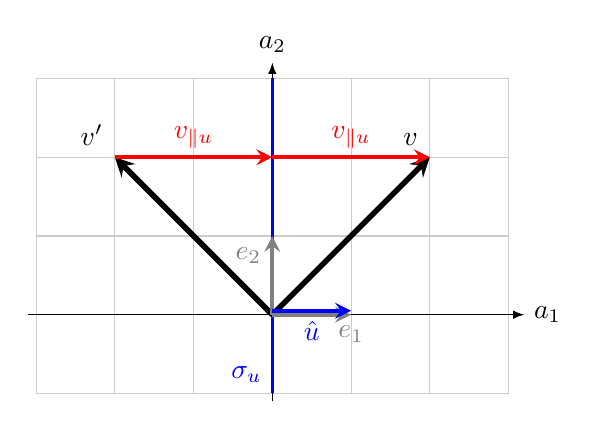
\begin{tikzpicture}[>=latex]
	\draw[thin,gray!40] (-3,-1) grid (3,3);
	\draw[->] (-3.1,0)--(3.2,0) node[right]{$a_1$};
	\draw[->] (0,-1.1)--(0,3.2) node[above]{$a_2$};
	\draw[blue, line width=1.0pt] (0,3)--(0,-1) node[anchor=south east]{$\sigma_u$};
	\draw[line width=2pt,black,-stealth](0,0)--(2,2) node[anchor=south east]{$\boldsymbol{v}$};
	\draw[line width=2pt,black,-stealth](0,0)--(-2,2) node[anchor=south east]{$\boldsymbol{v'}$};
	\draw[line width=1.5pt,gray,-stealth](0,0)--(1,0) node[anchor=north]{$\boldsymbol{e_1}$};
	\draw[line width=1.5pt,gray,-stealth](0,0)--(0,1) node[anchor=north east]{$\boldsymbol{e_2}$};
	\draw[line width=1.5pt,red,-stealth](0,2)--(2,2) node[xshift=-1cm, yshift=
	0.25cm]{$\boldsymbol{v_{\parallel u}}$};
	\draw[line width=1.5pt,red,-stealth](-2,2)--(0,2) node[xshift=-1cm, yshift=
	0.25cm]{$\boldsymbol{v_{\parallel u}}$};
	\draw[line width=1.5pt,blue,-stealth](0,0.05)--(1,0.05) node[xshift=-0.5cm, yshift=-0.25cm]{$\boldsymbol{\hat{u}}$};
	\end{tikzpicture}
	\caption{Spiegelung des Vektors $\mathbf{v}$ an der Spiegelebene $\sigma_u$ mit dem Normalenvektor $\mathbf{\hat{u}}$}
	\label{BildSpiegelung}
\end{figure}

\subsection{Spiegelung in der linearen Algebra}
Aus der linearen Algebra ist bekannt, dass man eine Spiegelung an einer Ebene wie in Abbildung \ref{BildSpiegelung} gezeigt wie folgt beschreiben kann.
\begin{definition}
	Die Abbildung der Spiegelung in der linearen Algebra mit dem Normalenvektor $\mathbf{\hat{u}}$ zur Spiegelebene ist
	\begin{equation} \label{RefLinAlg}
	\mathbf{v} = \mathbf{v_{\perp u}} + \mathbf{v_{\parallel u}} \enspace\mapsto\enspace \mathbf{v'} =  \mathbf{v_{\perp u}} - \mathbf{v_{\parallel u}} = \mathbf{v} - 2 \cdot \mathbf{v_{\parallel u}}.
	\end{equation}
\end{definition}
Es scheint für diese Formel \eqref{RefLinAlg} aber umständlich zu sein, weitere Spiegelungen mit weiteren Spiegelebenen anzufügen. Weil man $\mathbf{v_{\parallel u}}$ auch als Skalarprodukt $\mathbf{v_{\parallel u}} = \mathbf{\hat{u}} \cdot \mathbf{v}$ schreiben kann, ist es leicht, diese Abbildung auch als Matrix darzustellen. Sei $\mathbf{\hat{u}}$ ein Normalenvektor auf die Spiegelungsebene, also $\mathbf{\hat{u}}\perp \sigma_u$, und sei ausserdem normiert $|\mathbf{\hat{u}}| = 1$, dann kann die Spiegelung durch die Matrix
\begin{align*}
S = E - 2\mathbf{\hat{u}\hat{u}}^t
\end{align*}
beschrieben werden. In zwei und drei Dimensionen ergibt die Berechnung
\begin{align} \label{Spiegelmatrizen}
S_2 = \begin{pmatrix}
1-2u_1^2 & -2u_1u_2 \\
-2u_1u_2 & 1-2u_2^2
\end{pmatrix}\quad\text{und}\quad
S_3 = \begin{pmatrix}
1-2u_1^2 & -2u_1u_2 & -2u_1u_3\\
-2u_1u_2 & 1-2u_2^2 & -2u_2u_3\\
-2u_1u_3 & -2u_2u_3 & 1-2u_3^2\\
\end{pmatrix}.
\end{align}
Diese Spiegelmatrizen gehören der orthogonalen Matrizengruppe $S_n\in \text{O}(n)$ an.
\index{On@$\operatorname{O}(n)$}%
Die Matrizengruppe $\text{O}(n)$ hat die Eigenschaft $S_n^t S_n = E$, was bedeutet, dass die Länge und Winkel bei der Abbildung beibehalten bleiben. Zusätzlich sind die Spiegelmatrizen symmetrisch, es gilt $S_n^t = S_n$. Somit liefert zweimal dieselbe Spiegelung wieder die identische Abbildung, wie man aus
\begin{align*}
S_n^t S_n = S_n^2 = E
\end{align*}
schliessen kann.

\subsection{Spiegelung in der geometrische Algebra}
Wir definieren zuerst die Inverse eines Vektors, welche in dieser Form in der linearen Algebra nicht existiert.
\index{Inverse eines Vektors}%
\begin{definition}
	Die Inverse eines Vektors wird definiert als
	\begin{align} \label{InverseGA}
	\mathbf{u}^{-1} = \dfrac{\mathbf{u}}{|\mathbf{u}|^2}. 
	\end{align}
\end{definition}
Diese Definition ist sinnvoll, da wegen $\mathbf{u}^2 = |\mathbf{u}|^2$ folgt
\begin{align*}
\mathbf{uu}^{-1} = \mathbf{u} \frac{\mathbf{u}}{|\mathbf{u}|^2} = \frac{\mathbf{u}^2}{|\mathbf{u}|^2} = \frac{|\mathbf{u}|^2}{|\mathbf{u}|^2} = 1.
\end{align*}
Der Vektor $\mathbf{u}^{-1}$ in \eqref{InverseGA} ist also tatsächlich das inverse Element im Sinne des Produktes in der geometrischen Algebra.
Die geometrische Algebra leitet aus der obigen Formel \eqref{RefLinAlg} für eine Spiegelung eine einfache und intuitive Form her, welche auch für weitere Operationen erweitert werden kann.
\begin{definition}
	Die Abbildung der Spiegelung in der geometrischen Algebra mit dem senkrechten Vektor $\mathbf{u}$ zur Spiegelungsebene $\sigma_u$ ist 
	\begin{align}\label{RefGA}
	\mathbf{v} \enspace\mapsto\enspace \mathbf{v}' = -\mathbf{uvu}^{-1}.
	\end{align}
\end{definition}
Um zu überprüfen, ob die Spiegelungsgleichung \eqref{RefGA} wirklich eine Spiegelung ist, setzen wir zuerst in diese Gleichung $\mathbf{v} = \mathbf{v_{\perp u}} + \mathbf{v_{\parallel u}}$ ein. Wir bekommen somit
\begin{align*}
\mathbf{v}' = -\mathbf{uv_{\perp u}u}^{-1} - \mathbf{uv_{\parallel u}u}^{-1}.
\end{align*}
Danach können wir mit Hilfe der aus der Schlussfolgerung \eqref{uperpv} und \eqref{uparallelv} hergeleiteten Zusammenhänge
\begin{align*}
\mathbf{uv_{\perp u}} = -\mathbf{v_{\perp u}u} \quad\text{und}\quad \mathbf{uv_{\parallel u}}=\mathbf{v_{\parallel u}u},
\end{align*}
die Gleichung weiter umformen zu
\begin{align*}
\mathbf{v}' = -(-\mathbf{v_{\perp u}}\underbrace{\mathbf{u})\mathbf{u}^{-1}}_{1} -(\mathbf{v_{\parallel u}}\underbrace{\mathbf{u})\mathbf{u}^{-1}}_{1} = \mathbf{v_{\perp u}} - \mathbf{v_{\parallel u}}.
\end{align*}
Man sieht, dass das Resultat $\mathbf{v}' = \mathbf{v_{\perp u}} - \mathbf{v_{\parallel u}}$
gleichbedeutend zu der Definition \eqref{RefLinAlg} der Spiegelung ist.

Verwendet man für $\mathbf{u}$ nur einen Einheitsvektor $\mathbf{\hat{u}}$, wird die Gleichung \eqref{RefGA} zu
\begin{align}
\mathbf{v'} = -\mathbf{\hat{u}v\hat{u}}
\end{align}
vereinfacht.
Im Gegensatz zu den Abbildungen in der linearen Algebra, welche in
jeder anderen Dimension durch andere Matrizen \eqref{Spiegelmatrizen}
beschrieben werden müssen, ist es in der geometrischen Algebra immer
der gleiche Vorgehensweise.
Zudem ist diese kompakte Schreibweise in der linearen Algebra nicht
möglich, da bis auf das Vektorprodukt in drei Dimensionen keine
Multiplikation von Vektoren definiert ist.

%
% teil2.tex -- Beispiel-File für teil2 
%
% (c) 2020 Prof Dr Andreas Müller, Hochschule Rapperswil
%
\section{Rotation}
\rhead{Rotation}

Eine Rotation kann man aus zwei aufeinanderfolgenden Spiegelungen bilden. Das wird für einige zuerst eine verwirrende Aussage sein, da man aus den vorherig gezeigten Formeln annehmen könnte, dass die Spiegelung schon für eine Drehung ausreicht. Obwohl sich die Längen, Winkel und Volumen sich bei einer Spiegelung, wie bei einer Rotation, nicht ändert, sind sie doch verschieden, da die Orientierung bei der Spiegelung invertiert wird. Stellt man sich beispielsweise ein Objekt im Dreidimensionalen vor und spiegelt dieses an einer Fläche, dann ist es unmöglich nur durch eine Rotation (egal an welchem Punkt) das ursprüngliche Objekt deckungsgleich auf das Gespiegelte zu drehen. Hingegen ist es wiederum möglich ein zweifach gespiegeltes Objekt durch eine Drehung zu erreichen. Das liegt daran, da die Orientierung zweimal invertiert wurde.
\\(Hier wird noch ein Bild für das Verständnis eingefügt)

\begin{figure}
	\centering
	\begin{tikzpicture}
		\draw[thin,gray!40] (-3,-1) grid (3,3);
		\draw[<->] (-3,0)--(3,0) node[right]{$a_1$};
		\draw[<->] (0,-1)--(0,3) node[above]{$a_2$};
		\draw[line width=2pt,black,-stealth](0,0)--(2,2) node[anchor=south east]{$\boldsymbol{v}$};
		\draw[line width=1.5pt,blue,-stealth](0,0)--(0,2.5) node[anchor=south east]{$\boldsymbol{u}$};
		\draw[line width=2pt,black,-stealth](0,0)--(-2,2) node[anchor=south east]{$\boldsymbol{v'}$};
		\draw[line width=1.5pt,red,-stealth](0,0)--(-2.31, 0.957) node[anchor=south east]{$\boldsymbol{w}$};
		\draw[line width=2pt,black,-stealth](0,0)--(-2.828,0) node[anchor=south east]{$\boldsymbol{v''}$};
		\draw[line width=1.5pt,gray,-stealth](0,0)--(1,0) node[anchor=north]{$\boldsymbol{e_1}$};
		\draw[line width=1.5pt,gray,-stealth](0,0)--(0,1) node[anchor=north west]{$\boldsymbol{e_2}$};
		
		\coordinate (A) at (0,0);
		\coordinate (B) at (0,2.5);
		\coordinate (C) at (-2.31, 0.957);
		\tikzset{anglestyle/.style={angle eccentricity=1.25, draw,  thick, angle radius=1.25cm}}
		\draw pic ["$\theta$", anglestyle] {angle = B--A--C};
	\end{tikzpicture}
	\caption{Rotation des Vektors $\textbf{v}$ um $2\theta$}
	\label{BildRotation}
\end{figure}

\subsection{Linearen Algebra}
In der linearen Algebra haben wir Drehungen durch die Matrizen der Gruppe $\text{SO}(n)$ beschrieben. Beispielsweise besteht $\text{SO}(2)$  aus den Matrizen
\begin{align}
	D = 
	\begin{pmatrix}
		\cos(\alpha) & \sin(\alpha) \\
		-\sin(\alpha) & \cos(\alpha) 
	\end{pmatrix},\quad
	\alpha \in [0, 2\pi).
\end{align}
Diese Drehmatrizen gehören der speziellen orthogonalen Matrizengruppe $D\in \text{SO}(n) = \text{SL}_n(\mathbb{R})\enspace \cap \enspace \text{O}(n)$ an. $\text{SL}_n(\mathbb{R})$ beinhaltet die Matrizen mit scherenden Eigenschaften. Diese Drehmatrizen haben die Eigenschaft $D^t D = E \enspace \land \enspace \det(D)=1$. Da $\det(D) = 1$ und nicht $-1$ sein kann fallen alle Spiegelungen aus der Menge heraus. $\det(D) = -1$ bedeutet, dass eine Orientierungsinversion stattfindet.  
\\(BILD Mengen Spezieller Matrizen von Herrn Müller Präsentation)

\subsection{Geometrische Algebra}
Da wir jetzt aus der Geometrie wissen, dass eine Rotation durch zwei Spiegelungen gebildet werden kann, können wir die Rotation mit der Formel \eqref{RefGA} einfach herleiten.
\begin{satz}
	Eine Rotation 
	\begin{align} \label{rotGA}
		\mathbf{v}'' = \mathbf{wv}'\mathbf{w}^{-1} = \mathbf{w}(\mathbf{uvu}^{-1})\mathbf{w}^{-1} = (\mathbf{wu})\mathbf{v}(\mathbf{u}^{-1}\mathbf{w}^{-1})
	\end{align}
	lässt sich durch zwei nacheinander auf einen Vektor $\mathbf{v}$ angewendete Spiegelungen beschreiben.
\end{satz}
Die Vektoren $\mathbf{w}$ und $\mathbf{u}$ bilden hier wiederum die Spiegelachsen. Diese Formel versuchen wir jetzt noch durch Umstrukturierung zu verbessern. 
\subsubsection{Exponentialform}
Dazu leiten wir zuerst die Exponentialform eines Vektors her. Es wird dabei zur Vereinfachung davon ausgegangen, dass alle Vektoren $\mathbf{w}, \mathbf{u}, \mathbf{v}$ in der $\mathbf{e}_{12}$ Ebene liegen. Weitere Drehungen können in höheren Dimensionen durch Linearkombinationen von Drehungen in den $\mathbf{e}_{ij}, i\not=j$ Ebenen erreicht werden. Für die Herleitung erweitern wir nun als erstes die Polarform
\begin{align}
	\mathbf{w} = |\mathbf{w}| \left(\cos(\theta_w) \mathbf{e}_1 + \sin(\theta_w) \mathbf{e}_2\right)
\end{align}
eines Vektors mit $\mathbf{e}_1^2 = 1$ beim Sinus
\begin{align}\label{e1ausklammern}
	\mathbf{w} &= |\mathbf{w}| \left(\cos(\theta_w) \mathbf{e}_1 + \sin(\theta_w) \mathbf{e}_1\mathbf{e}_1\mathbf{e}_2\right), 
\end{align}
um dann $\mathbf{e}_1$
\begin{align}
	\mathbf{w} = |\mathbf{w}|\mathbf{e}_1\left(\cos(\theta_w)+ \sin(\theta_w) \mathbf{e}_{12}\right) \label{ExponentialGA}
\end{align}
ausklammern zu können. Die Ähnlichkeit des Klammerausdrucks zu der Eulerschen Formel bei den Komplexen Zahlen ist nun schon gut erkennbar. Versuchen wir nun mithilfe der Reihenentwicklungen
\begin{align}
	\sin(\theta_w)\mathbf{e}_{12}&=\sum _{n=0}^{\infty }(-1)^{n}{\frac {\theta_w^{2n+1}}{(2n+1)!}}\mathbf{e}_{12} =\theta_w\mathbf{e}_{12}-{\frac {\theta_w^{3}}{3!}}\mathbf{e}_{12}+{\frac {\theta_w^{5}}{5!}}\mathbf{e}_{12}-\cdots \\
	\cos(\theta_w)&=\sum _{n=0}^{\infty }(-1)^{n}{\frac {\theta_w^{2n}}{(2n)!}} =1-{\frac {\theta_w^{2}}{2!}}+{\frac {\theta_w^{4}}{4!}}-\cdots
\end{align}
den Zusammenhang auch hier herzustellen. Verwenden wir jetzt noch die Eigenschaft, dass $\mathbf{e}_{12}^2=-1, \enspace\mathbf{e}_{12}^3=-\mathbf{e}_{12}, \dots$, bei dem Klammerausdruck in Formel \eqref{ExponentialGA}
\begin{align}
	\cos(\theta_w)+ \sin(\theta_w) \mathbf{e}_{12} &= 1+\theta_w\mathbf{e}_{12}-{\frac {\theta_w^{2}}{2!}}-{\frac {\theta_w^{3}}{3!}}\mathbf{e}_{12}+{\frac {\theta_w^{4}}{4!}}+{\frac {\theta_w^{5}}{5!}}\mathbf{e}_{12}-\cdots\\
	&= 1 \mathbf{e}_{12}^0+\theta_w\mathbf{e}_{12}^1+{\frac {\theta_w^{2}}{2!}}\mathbf{e}_{12}^2+{\frac {\theta_w^{3}}{3!}}\mathbf{e}_{12}^3+{\frac {\theta_w^{4}}{4!}}\mathbf{e}_{12}^4+{\frac {\theta_w^{5}}{5!}}\mathbf{e}_{12}^5+\cdots
	\label{ExponentialGA2}
\end{align}
dann sieht man die Übereinstimmung mit der Reihenentwicklung der Exponentialfunktion
\begin{align}
	&e^{\theta_w\mathbf{e}_{12}}=\sum _{n=0}^{\infty }{\frac {(\theta_w\mathbf{e}_{12})^{n}}{n!}}={\frac {(\theta_w\mathbf{e}_{12})^{0}}{0!}}+{\frac {(\theta_w\mathbf{e}_{12})^{1}}{1!}}+{\frac {(\theta_w\mathbf{e}_{12})^{2}}{2!}}+{\frac {(\theta_w\mathbf{e}_{12})^{3}}{3!}}+\cdots\\
	&\Rightarrow \mathbf{w} = |w|\mathbf{e}_1 e^{\theta_w \mathbf{e}_{12}} = |w|\mathbf{e}_1\left(\cos(\theta_w)+ \sin(\theta_w) \mathbf{e}_{12}\right).
\end{align}
Man kann die Exponentialform des Vektors ähnlich wie die der komplexen Zahlen interpretieren. Der Einheitsvektor $\mathbf{e}_1$ wird um die Länge $|\mathbf{w}|$ gestreckt und um $\theta_w$ gedreht.
Bei den komplexen Zahlen würden man vom Punkt 1 anstatt $\mathbf{e}_1$ ausgehen.
\subsubsection{Vektormultiplikation}
Nun werden wir das Produkt von zwei Vektoren $\mathbf{wu}$
\begin{align}
	\mathbf{wu} = |\mathbf{w}|\mathbf{e}_1 e^{\theta_w \mathbf{e}_{12}}|\mathbf{u}|\mathbf{e}_1 e^{\theta_u \mathbf{e}_{12}}
\end{align}
so umformen, dass wir eine bessere Darstellung erhalten. Wir tauschen dafür zuerst beim Vektor $\mathbf{w}$ die Reihenfolge von 
$\mathbf{e}_1$ mit dem Exponentialterm $e^{\theta_w \mathbf{e}_{12}}$, indem wir bei der Gleichung \eqref{e1ausklammern}, anstatt mit $\mathbf{e}_1\mathbf{e}_1\mathbf{e}_2$ mit $\mathbf{e}_2\mathbf{e}_1\mathbf{e}_1$ erweitern
\begin{align} 
	\mathbf{w} &= |\mathbf{w}|\left(\cos(\theta_w)+ \sin(\theta_w) \mathbf{e}_2\mathbf{e}_1\right)\mathbf{e}_1\\
	&= |\mathbf{w}|e^{\theta_w \mathbf{e}_{21}}\mathbf{e}_1\\
	&= |\mathbf{w}|e^{-\theta_w \mathbf{e}_{12}}\mathbf{e}_1
\end{align}
und umstrukturiert wieder in die Vektorproduktformel einsetzen
\begin{align}
	\mathbf{wu} = |\mathbf{w}||\mathbf{u}|e^{-\theta_w \mathbf{e}_{12}}\mathbf{e}_1\mathbf{e}_1 e^{\theta_u \mathbf{e}_{12}}\\
	\mathbf{wu} = |\mathbf{w}||\mathbf{u}|e^{(\theta_u-\theta_w) \mathbf{e}_{12}}.
\end{align}
Der Term $\mathbf{u}^{-1}\mathbf{w}^{-1}$
\begin{align}
	\mathbf{u}^{-1}\mathbf{w}^{-1} = \dfrac{1}{|\mathbf{w}||\mathbf{u}|}e^{(\theta_w-\theta_u) \mathbf{e}_{12}}
\end{align}
kann durch die selbe Methode zusammengefasst werden.
Wenn wir den Winkel zwischen den Vektoren  $\mathbf{w}$ und $\mathbf{u}$ als $\theta = \theta_w - \theta_u$ definieren erhalten wir
\begin{align}\label{wuExpo}
	\mathbf{wu} = |\mathbf{w}||\mathbf{u}|e^{-\theta \mathbf{e}_{12}}\\
	\mathbf{u}^{-1}\mathbf{w}^{-1} = \dfrac{1}{|\mathbf{w}||\mathbf{u}|}e^{\theta \mathbf{e}_{12}} \label{wuExpoInv}
\end{align}
die finale Form der Vektorprodukte.
\subsubsection{Umstrukturierte Drehungsgleichung}
Setzten wir nun unsere neuen Erkenntnisse in die Gleichung \eqref{rotGA} ein
\begin{align}
	\mathbf{v''} = (|\mathbf{w}||\mathbf{u}|e^{-\theta \mathbf{e}_{12}}) \mathbf{v}( \dfrac{1}{|\mathbf{w}||\mathbf{u}|}e^{\theta \mathbf{e}_{12}}),
\end{align}
erhalten wir durch die Kürzungen der Längen die vereinfachte Drehungsgleichung
\begin{align}
	\mathbf{v''} = e^{-\theta \mathbf{e}_{12}} v e^{\theta \mathbf{e}_{12}}.
\end{align}

Wir wissen nun, dass das diese beidseitige Multiplikation die Länge von $\mathbf{v}$ nicht verändert, da sich die Längen von $\mathbf{w}$ und $\mathbf{u}$ kürzen. Betrachten wir nun den Effekt der Exponentialterme auf $\mathbf{v}$. Dabei Teilen wir den Vektor $\mathbf{v}$ auf in einen Anteil $\mathbf{v_\parallel}$, welcher auf der Ebene $\mathbf{e}_{12}$ liegt, und einen Anteil $\mathbf{v_\perp}$, welcher senkrecht zu der Ebene steht. Wir bekommen durch Einsetzten nun diese Form
\begin{align} \label{RotAufPerpPar}
	\mathbf{v}'' = e^{-\theta \mathbf{e}_{12}} (\mathbf{v_\perp + v_\parallel}) e^{\theta \mathbf{e}_{12}} = e^{-\theta \mathbf{e}_{12}} \mathbf{v_\perp} e^{\theta \mathbf{e}_{12}} + e^{-\theta \mathbf{e}_{12}} \mathbf{v_\parallel} e^{\theta \mathbf{e}_{12}}.
\end{align}
Auf eine allgemeine Herleitung wird hier zwar verzichtet, aber man kann zeigen, dass die Reihenfolge so umstrukturiert werden kann
\begin{align}
	\mathbf{v}'' = \mathbf{v_\perp} e^{-\theta \mathbf{e}_{12}}  e^{\theta \mathbf{e}_{12}} +  \mathbf{v_\parallel} e^{-(-\theta) \mathbf{e}_{12}} e^{\theta \mathbf{e}_{12}},
\end{align}
dass der Winkel beim parallelen Anteil negiert wird. An der Zusammengefassten Gleichung
\begin{align}\label{RotParPerp}
	\mathbf{v}'' = \mathbf{v_\perp} +  \mathbf{v_\parallel} e^{2\theta \mathbf{e}_{12}}
\end{align}
kann man sehen, dass nur der parallele Anteil $\mathbf{v_\parallel}$ des Vektors $\mathbf{v}$ auf der Ebene $\mathbf{e}_{12}$ um $2\theta$ gedreht wird. Der senkrechte Anteil $\mathbf{v_\perp}$ bleibt gleich. Wichtig dabei zu sehen ist, dass nur der Winkel zwischen den Vektoren $\mathbf{w}$ und $\mathbf{u}$ von Bedeutung ist. Die Länge und Richtung der einzelnen Vektoren spielt keine Rolle. Zeigen wir nun diese Eigenschaften an einem Beispiel
\begin{beispiel} 
	Gegeben sei ein Vektor $\mathbf{v} = 1\mathbf{e}_1 + 2\mathbf{e}_2 + 3\mathbf{e}_3$ mit zur $\mathbf{e}_{12}$-Ebene parallelen Anteil $\mathbf{v_\parallel} = 1\mathbf{e}_1 + 2\mathbf{e}_2$ und senkrechten Anteil $\mathbf{v_\perp} = 3\mathbf{e}_3$. Zusätzlich sind die Spiegelachsen $\mathbf{u} = \mathbf{e}_1$ und $\mathbf{w} = 2\mathbf{e}_2$ gegeben. Gesucht ist der rotierte Vektor $\mathbf{v}''$. Bestimmen wir als erstes das Vektorprodukt $\mathbf{wu}$
	\begin{align}
		\mathbf{wu} = (2\mathbf{e}_2)(\mathbf{e}_1) = -2\mathbf{e}_{12}
	\end{align}
	und das Produkt der Inversen $\mathbf{u}^{-1}\mathbf{w}^{-1}$
	\begin{align}
		\mathbf{u}^{-1}\mathbf{w}^{-1} = (\dfrac{\mathbf{e}_1}{1^2})(\dfrac{2\mathbf{e}_2}{2^2}) = \dfrac{1}{2}\mathbf{e}_{12}.
	\end{align}
	Der rotierte Vektor $\mathbf{v}''$ können wir nun durch das einsetzten und auflösen der Produkte in die Gleichung \eqref{rotGA}
	\begin{align}
		\mathbf{v}'' = (\mathbf{wu})\mathbf{v}(\mathbf{u}^{-1}\mathbf{w}^{-1}) &= (-2e_{12})(1\mathbf{e}_1 + \mathbf{e}_2 + 1\mathbf{e}_3)(\dfrac{1}{2}\mathbf{e}_{12})\\
		&= (2\mathbf{e}_2-2\mathbf{e}_1-2\mathbf{e}_{123})(\dfrac{1}{2}\mathbf{e}_{12})\\
		&= -1\mathbf{e}_1 - 1\mathbf{e}_2 + 1\mathbf{e}_3
	\end{align}
	finden. Aus dem Resultat $\mathbf{v}''= -1\mathbf{e}_1 + 1\mathbf{e}_2 + 1\mathbf{e}_3$ können wir bestätigen, dass
	\begin{itemize}
		\item die Länge $|\mathbf{v}| = \sqrt{3}$ zur Länge $|\mathbf{v}''|=\sqrt{3}$ gleich blieb.
		\item sich der parallele Anteil $\mathbf{v_\parallel}'' = -1\mathbf{e}_1 - 1\mathbf{e}_2$ gedreht hat und der senkrechte Anteil $\mathbf{v_\perp}'' = 1\mathbf{e}_3$ unverändert blieb.
		\item der parallele Teil sich genau um $2\theta=180$° gedreht hat. $\theta$ kann übrigens durch die Umformung des Produkt $\mathbf{wu}$ in die Exponentialschreibweise
		\begin{align}
			&\mathbf{wu} = -2\mathbf{e}_{12} = 2(0-1\mathbf{e}_{12})=2(\cos(\dfrac{-\pi}{2} + \sin(\dfrac{-\pi}{2})\mathbf{e}_{12})) = 2e^{(-\pi/2)\mathbf{e}_{12}}
		\end{align}
		durch einen Vergleich mir der Formel \eqref{wuExpo}
		\begin{align}
			\theta = -(\dfrac{-\pi}{2}) = \dfrac{\pi}{2}
		\end{align}
		ausgelesen werden.
	\end{itemize}
\end{beispiel}
%
% teil3.tex -- Beispiel-File für Teil 3
%
% (c) 2020 Prof Dr Andreas Müller, Hochschule Rapperswil
%
\section{Komplexe Zahlen}
\rhead{Komplexe Zahlen}

Die komplexen Zahlen finden eine Vielzahl von Anwendungsgebiete in den Ingenieurwissenschaften. Das liegt daran, weil die komplexen Zahlen Rotationen und Schwingungen gut beschreiben können. Nachdem vorherigen Kapitel überrascht es wahrscheinlich nicht viele, dass es möglich ist komplexe Zahlen in der geometrischen Algebra darzustellen. Sie können durch die geraden Grade der 2 Dimensionalen geometrischen Algebra vollständig beschrieben werden: $G_2^+(\mathbb{R}) \cong \mathbb{C}$. Das bedeutet eine komplexe Zahl kann durch ein Skalar (Grad 0) und einem Bivektor (Grad 2) dargestellt werden. Als Abkürzung nehme ich die Bezeichnung $\mathbf{g}_n \in  G_2^+(\mathbb{R})$.
\begin{align}
	a_0 + a_1 j \cong a_0 + a_1 \mathbf{e}_{12} = \mathbf{g}_n\quad a_0, a_1 \in \mathbb{R}
\end{align}
oder in Polarform.
\begin{align}
	|r|e^{\theta j} \cong |r|e^{\theta \mathbf{e}_{12}} = \mathbf{g}_n; \quad r, \theta \in \mathbb{R}
\end{align}
Man beachte, dass wenn wir, wie bei den komplexen Zahlen, Elemente von $G_2^+(\mathbb{R})$ miteinander Multiplizieren, ist es nicht, wie im Kapitel Rotation bei der Formel (\ref{rotGA})beschrieben, eine Multiplikation von zwei $g_n$ mit einem Vektor. Im zweidimensionalen bewirken beide Multiplikationen grundsätzlich das Gleiche (eine Drehstreckung), aber die Multiplikation von mehreren $g_n$ ist kommutativ, wie wir es von den komplexen Zahlen kennen.
\begin{align}
	\mathbf{g}_1\mathbf{g}_2 = \mathbf{g}_2\mathbf{g}_1 \quad&\Leftrightarrow\quad (a + b \mathbf{e}_{12})(f + g \mathbf{e}_{12}) = (f + g \mathbf{e}_{12})(a + b \mathbf{e}_{12})\\
	\mathbf{g}_1\mathbf{v}\mathbf{g}_2\not= \mathbf{g}_2\mathbf{v}\mathbf{g}_1 \quad&\Leftrightarrow\quad(a + b \mathbf{e}_{12})(x\mathbf{e}_1+y\mathbf{e}_2)(f + g \mathbf{e}_{12}) \not= (a + b \mathbf{e}_{12})(f + g \mathbf{e}_{12})(x\mathbf{e}_1+y\mathbf{e}_2)
\end{align}
Um später die Auswirkung der Quaternionen besser zu verstehen, möchte ich kurz darauf eingehen, was ein $g_n$ für eine Auswirkung auf einen Vektor hat.
Wir kennen diesen Effekt schon von den komplexen Zahlen. Wenn eine komplexe Zahl $c_1=a+bj$ mit einer zweiten $c_2=f+gj$ multipliziert wird, dann kann man diese so aufteilen.
\begin{align}
	c = c_1\cdot c_2 = (a + bj)(d + ej) = f\cdot(a+bj) + gj\cdot(a+bj)
\end{align}
Dabei ist $f\cdot(a+bj)$ die jetzige komplexe Zahl $c_1$ um den Faktor $f$ steckt und $gj\cdot(a+bj)$ die um 90° im Gegenuhrzeigersinn gedrehte Zahl $c_2$ um den Faktor $g$ streckt. Diese Anteile addiert ergeben, dann den um $c_2$ dreh-gestreckten Vektor $c_1$. Die wirklichen Vorteile der geometrischen Algebra werden sich aber erst bei den Quaternionen zeigen.
%
% teil3.tex -- Beispiel-File für Teil 3
%
% (c) 2020 Prof Dr Andreas Müller, Hochschule Rapperswil
%
\section{Quaternionen}
\rhead{Quaternionen}

Wie die komplexen Zahlen eine Erweiterung der reellen Zahlen sind, sind die Quaternionen eine Erweiterung der komplexen Zahlen für den dreidimensionalen Raum. Sie haben, wie die komplexen Zahlen, eine dreh-streckende Eigenschaft.
Sie finden beispielsweise in der Computergrafik und Robotik Anwendung.
Die Quaternionen
\begin{align}
	q = w + xi + yj + zk \quad w,x,y,z \in \mathbb{R}\enspace q \in \mathbb{H}
\end{align}
können dabei eine Drehstreckung mit
\begin{align} \label{QuatRot}
	\begin{split} 
		v \mapsto v'' = qvq^{-1}
	\end{split}
\end{align}
erreichen, falls $q,v,q^{-1} \in \mathbb{H}$ und die Zusammenhänge
\begin{align}
	\operatorname{Re}(q) = \operatorname{Re}(q^{-1})\quad \operatorname{Im}(q) = -\operatorname{Im}(q^{-1})
\end{align}
gelten. Auffallend ist bei der abbildenden Funktion \eqref{QuatRot} schon die Ähnlichkeit zu \eqref{rotGA} im Kapitel Rotation. Man könnte sich nun fragen wieso es drei imaginäre Einheiten $i,j,k$ gibt und nicht zwei, was doch näherliegender wäre. Der Grund liegt darin, weil es in der dritten Dimension drei Drehachsen gibt, anstatt nur eine. Wie im Kapitel Rotation beschrieben können wir auch hier die drei Drehungen durch Linearkombinationen von drei Bivektoren beschreiben. In der geometrischen Algebra ist es leicht herauszufinden wie viele Imaginärteile für jede weitere Dimension existieren. Dabei muss man nur die Anzahl der unabhängigen Bivektoren ermitteln. In der vierten Dimension würden es beispielsweise durch alle Vektorkombinationen von $\mathbf{e}_1, \mathbf{e}_2,\mathbf{e}_3, \mathbf{e}_4$ insgesamt 8 Bivektoren existieren (Nicht 16, da $\mathbf{e}_{ij} = -\mathbf{e}_{ji}$ nicht unabhängig voneinander sind).

Ohne die geometrische Algebra, haben wir jetzt aber leider ein kleines Problem. Für die Darstellung der Quaternionen bräuchten wir insgesamt vier Achsen. Drei für die imaginären Einheiten und eine für die reelle Einheit. Ein weiterer Nachteil in visueller Hinsicht entsteht beim Anwenden eines Quaternion auf einen Vektor. Sie befinden sich nicht im gleichen Raum und müssen zuerst durch
\begin{align}
	\mathbf{v} = x\mathbf{\hat{x}} + y\mathbf{\hat{y}} + z \mathbf{\hat{z}} \in \mathbb{R}^3 \enspace\mapsto\enspace v = 0 + xi + yj + zk \in \mathbb{H}
\end{align}
ineinander umgewandelt werden, um damit zu rechnen.

\subsection{Geometrische Algebra}
Die geometrische Algebra kann beide Probleme beheben. Die Quaternionen können, wie schon im zweidimensionalen Fall durch die gerade Grade $G_3^+(\mathbb{R}) \cong \mathbb{H}$ dargestellt werden. Da wir uns jetzt aber in $G_3(\mathbb{R})$ befinden haben wir drei Basisvektoren $\mathbf{e}_1, \mathbf{e}_2, \mathbf{e}_3$ und können somit drei Bivektoren $\mathbf{e}_{12}, \mathbf{e}_{23}, \mathbf{e}_{31}$ bilden.
\begin{definition}
	Die Multivektoren mit Drehstreckenden Eigenschaften in $G_3(\mathbb{R})$ sind
	\begin{align}
		\mathbf{q} = w + x\mathbf{e}_{12} + y\mathbf{e}_{23} + z\mathbf{e}_{31} \quad w,x,y,z \in \mathbb{R}\enspace \mathbf{q} \in \mathbb{G}_3^+.
	\end{align}
\end{definition}

Die Probleme werden dadurch gelöst, da wir die Bivektoren im Raum nicht durch einzelne Achsen darstellen müssen, sondern sie als eine orientiere Fläche darstellen können. Anstatt die Vektoren in Quaternionen umzurechnen, können wir jetzt die Vektoren separat im gleichen Raum, wie in Abbildung \ref{BildQuaternionen} gezeigt, darstellen. 
\begin{figure}
	\centering
	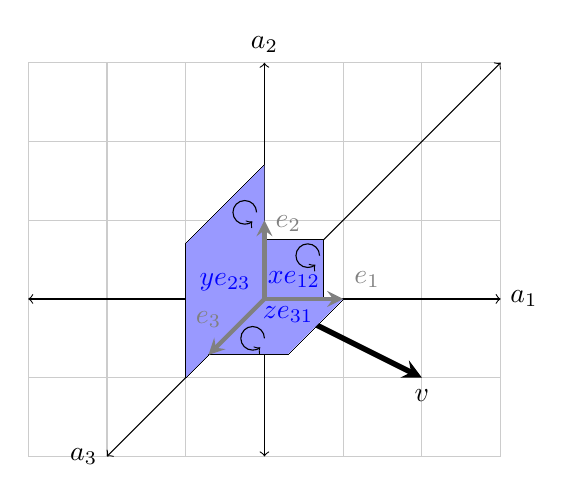
\begin{tikzpicture}
		% Koordinatensystem
		\draw[thin,gray!40] (-3,-2) grid (3,3);
		\draw[<->] (-3,0)--(3,0) node[right]{$a_1$};
		\draw[<->] (0,-2)--(0,3) node[above]{$a_2$};
		\draw[<->] (3,3)--(-2,-2) node[left]{$a_3$};
		
		% v Vektor
		\draw[line width=2pt,black,-stealth](0,0)--(2,-1) node[anchor=north]{$\boldsymbol{v}$};
		
		% q Quaternion
		\draw[line width=0,fill=blue!40] (0,0)--(0.75,0)--(0.75,0.75)--(0,0.75)
		node[xshift=0.375cm, yshift=-0.5cm, blue]{$x\boldsymbol{e_{12}}$};
		\draw[->] (0.7,0.55) arc (0:310:0.15);
		
		\draw[line width=0,fill=blue!40] (0,0)--(-1,-1)--(-1,0.71)--(0,1.71)
		node[xshift=-0.5cm, yshift=-1.5cm, blue]{$y\boldsymbol{e_{23}}$};
		\draw[->] (-0.1,1.1) arc (0:310:0.15);
		
		\draw[line width=0,fill=blue!40] (0,0)--(-0.71,-0.71)--(0.29,-0.71)--(1,0)
		node[xshift=-0.7cm, yshift=-0.2cm, blue]{$z\boldsymbol{e_{31}}$};
		\draw[->] (0,-0.5) arc (0:310:0.15);
		
		% Basisvektoren
		\draw[line width=1.5pt,gray,-stealth](0,0)--(1,0) node[anchor=south west]{$\boldsymbol{e_1}$};
		\draw[line width=1.5pt,gray,-stealth](0,0)--(0,1) node[anchor=north west, yshift=0.2cm]{$\boldsymbol{e_2}$};
		\draw[line width=1.5pt,gray,-stealth](0,0)--(-0.71,-0.71) node[anchor=south, yshift=0.2cm]{$\boldsymbol{e_3}$};
	\end{tikzpicture}
	\caption{Darstellung eines Quaternion $\mathbf{q}$ und eines Vektors $\mathbf{v}$ im selben Raum}
	\label{BildQuaternionen}
\end{figure}
Wie schon im zweidimensionalen Fall \eqref{GAdrehstreck} beschreibt im dreidimensionalen Fall mit drei Bivektoren
\begin{align}
	\mathbf{qv} &= (w + x\mathbf{e}_{12} + y\mathbf{e}_{23} + z\mathbf{e}_{31})(a\mathbf{e}_1+b\mathbf{e}_2+c\mathbf{e}_3)\\
	&= \underbrace{w(a\mathbf{e}_1+b\mathbf{e}_2+c\mathbf{e}_3)}_{w\mathbf{v}} + \underbrace{x(-a\mathbf{e}_2+b\mathbf{e}_1}_{x\mathbf{v}_{\angle 90^\circ, \parallel \mathbf{e}_{12}}}+c\mathbf{e}_{123}) + \underbrace{y(-b\mathbf{e}_3+c\mathbf{e}_2}_{y\mathbf{v}_{\angle 90^\circ, \parallel \mathbf{e}_{23}}}+a\mathbf{e}_{123}) + \underbrace{z(a\mathbf{e}_3-c\mathbf{e}_1}_{z\mathbf{v}_{\angle 90^\circ, \parallel \mathbf{e}_{31}}}-b\mathbf{e}_{123})
\end{align}
jeder Bivektoranteil, um wie viel der um 90° gedrehte zu der Ebene parallele Teil des Vektors gestreckt wird. Dabei dreht jeder Bivektor den Vektor um eine andere Achse und man sieht die dreh-streckende Eigenschaft ähnlich zu den komplexen Zahlen. Der störende Trivektoranteil $(xc+ya+zb)\mathbf{e}_{123}$ bekommt man aber nur weg, indem man noch wie in der Rotationsformel \eqref{QuatRot} den Inversen Quaternion $\mathbf{q}^{-1}$ anschliessend multipliziert, wobei die dreh-gestreckten parallelen Anteile nochmals um den gleichen Faktor dreh-gestreckt werden. Da nur so der Trivektoranteil wegfällt, sieht man, dass die Rotationsformel, der einzige Vernünftige weg ist, mit Quaternionen zu arbeiten.

In der Computergraphik und Robotik macht eine Drehstreckung aber nicht viel Sinn. Wieso sollte ein Objekt bei einer Drehung zusätzlich noch grösser werden? Darum verwendet man sogenannte Einheitsquaternionen, welche den Betrag $|\mathbf{q}|=1$ haben und somit rotieren sie die Objekte bzw. Vektoren lediglich.
\begin{definition}
	Die Einheitsquaternionen sind definiert als
	\begin{align}
		\mathbf{q} = \cos(\alpha) + sin(\alpha)(\tilde{x}\mathbf{e}_{12} + \tilde{y}\mathbf{e}_{23} + \tilde{z}\mathbf{e}_{31})
	\end{align}
\end{definition}
Zudem setzten wir $\tilde{x}^2+\tilde{y}^2+\tilde{z}^2=1$, damit
\begin{align}
	|\mathbf{q}| = \sqrt{cos(\alpha)^2 + sin(\alpha)^2(\tilde{x}^2+\tilde{y}^2+\tilde{z}^2) } = \sqrt{cos(\alpha)^2 + sin(\alpha)^2} = 1.
\end{align}
Der Winkel $\alpha$ beschreibt dabei, wie im Bild \ref{BildQuaternionBeispiel2} gezeigt den halben Winkel, um welchen der parallelen Anteil $\mathbf{v_{\parallel}}$ des Vektors $\mathbf{v}$ zur kombinierten Bivektorebene $sin(\alpha)^2(\tilde{x}\mathbf{e}_{12} + \tilde{y}\mathbf{e}_{23} + \tilde{z}\mathbf{e}_{31})$ gedreht wird.

Um einen Vektor zu drehen, verwendet man die in Kapitel Rotation hergeleitete Formel 
\begin{align} \label{QuatRotGA}
	\begin{split} 
		\mathbf{v}'' = \mathbf{qvq}^{-1},
	\end{split}
\end{align}
wobei wie auch schon bei den Quaternionen gelten muss, dass
\begin{align} \label{GAReIm}
	\operatorname{Re}(\mathbf{q}) = \operatorname{Re}(\mathbf{q}^{-1}) \enspace\text{und}\enspace \operatorname{Im}(\mathbf{q}) = -\operatorname{Im}(\mathbf{q}^-1).
\end{align}
Der Grund für die Zusammenhänge \eqref{GAReIm} kann man durch die hergeleitete vereinfachte Rotationsformel \eqref{GAvereinfRot} sehen, weil durch den negierten Winkel $\theta$ der Reelle bzw. Grad 0 Anteil
\begin{align}
	\operatorname{Re}(e^{-\theta \mathbf{e}_{12}}) = \operatorname{Re}(e^{\theta \mathbf{e}_{12}})
\end{align}
und der Imaginäre bzw. Grad 2 Anteil
\begin{align}
	\operatorname{Im}(e^{-\theta \mathbf{e}_{12}}) = -\operatorname{Im}(e^{\theta \mathbf{e}_{12}})
\end{align}
ist. Durch die geometrische Algebra sieht man nun wieso es wichtig ist bei Quaternionen für eine reine Drehstreckung mit $\mathbf{q}$ und $\mathbf{q}^{-1}$ beidseitig zu multiplizieren, sonst werden die senkrechten Anteile zu den Bivektorebenen ebenfalls beeinflusst, wie man im Kapitel Rotation bei der Formel (\ref{RotAufPerpPar}) sehen kann.
\begin{beispiel}
	Eine Drehung eines Vektors $\mathbf{v}= 1\mathbf{e}_2$ um 90 Grad um die $\mathbf{e}_1$-Achse und danach 90 Grad um die $\mathbf{e}_2$-Achse. Dafür nehmen wir zuerst einen Einheitsquaternion 
	\begin{align}
		\mathbf{q}_{23} &= \cos(\pi/4) + sin(\pi/4)(1\mathbf{e}_{23}) =  e^{(\pi/4)\mathbf{e}_{23}} &= \textstyle{\frac{\sqrt{2}}{2}}(1 + \mathbf{e}_{23})\\
		\mathbf{q}_{23}^{-1} &&= \textstyle{\frac{\sqrt{2}}{2}} (1- \mathbf{e}_{23})
	\end{align}
	welcher um die $\mathbf{e}_{2}$-$\mathbf{e}_{3}$-Ebene um 90 Grad dreht und danach Einheitsquaternion 
	\begin{align}
		\mathbf{q}_{31} &= \cos(\pi/4) + sin(\pi/4)(1\mathbf{e}_{31}) =  e^{(\pi/4)\mathbf{e}_{31}} &= \textstyle{\frac{\sqrt{2}}{2}}(1 + \mathbf{e}_{31})\\
		\mathbf{q}_{31}^{-1} &&= \textstyle{\frac{\sqrt{2}}{2}}(1 - \mathbf{e}_{31})
	\end{align}
	welcher um die $\mathbf{e}_{3}$-$\mathbf{e}_{1}$-Ebene  um 90 Grad dreht. Um die vollständige Rotation zu beschreiben können die  Einheitsquaternion multipliziert werden, wobei die Reihenfolge der Ausführung beachtet werden muss. Somit ist
	\begin{align} \label{FormelBeispielQuaternion}
		\mathbf{q} &= \mathbf{q}_{31}\mathbf{q}_{23} = \textstyle{\frac{\sqrt{2}}{2}}(1 + \mathbf{e}_{31})\textstyle{\frac{\sqrt{2}}{2}}(1 + \mathbf{e}_{23}) &= \textstyle{\frac{1}{2}}(1 + \mathbf{e}_{31} + \mathbf{e}_{23} + \mathbf{e}_{12})\\
		\mathbf{q}^{-1} &= \mathbf{q}_{23}^{-1}\mathbf{q}_{31}^{-1} = \textstyle{\frac{\sqrt{2}}{2}} (1- \mathbf{e}_{23})\textstyle{\frac{\sqrt{2}}{2}}(1 -\mathbf{e}_{31}) &= \textstyle{\frac{1}{2}}(1 - \mathbf{e}_{31} - \mathbf{e}_{23} - \mathbf{e}_{12}).
	\end{align}
	Wenn wir nun den Quaternion $\mathbf{q}$ auf den Vektor $\mathbf{v}$ anwenden
	\begin{align}
		\mathbf{v}'' = \mathbf{qvq}^{-1} &= \textstyle{\frac{1}{2}}(1 + \mathbf{e}_{31} +  \mathbf{e}_{23} +  \mathbf{e}_{12})(1\mathbf{e}_2)\textstyle{\frac{1}{2}}(1 - \mathbf{e}_{31} -  \mathbf{e}_{23} -  \mathbf{e}_{12})\\ 
		&= \textstyle{\frac{1}{4}}(\mathbf{e}_2 +  \mathbf{e}_{123} -  \mathbf{e}_3 +  \mathbf{e}_1)(1 - \mathbf{e}_{31} -  \mathbf{e}_{23} -  \mathbf{e}_{12})\\
		&= (\textstyle{\frac{1}{4}} + \textstyle{\frac{1}{4}} + \textstyle{\frac{1}{4}} + \textstyle{\frac{1}{4}})\mathbf{e}_1 + (\textstyle{\frac{1}{4}} + \textstyle{\frac{1}{4}} - \textstyle{\frac{1}{4}} - \textstyle{\frac{1}{4}})\mathbf{e}_2 +\\ &(-\textstyle{\frac{1}{4}} + \textstyle{\frac{1}{4}} - \textstyle{\frac{1}{4}} + \textstyle{\frac{1}{4}})\mathbf{e}_3 + (\textstyle{\frac{1}{4}} - \textstyle{\frac{1}{4}} - \textstyle{\frac{1}{4}} + \textstyle{\frac{1}{4}})\mathbf{e}_{123}\\
		&= 1e_1 
	\end{align}
	Anders betrachtet könnte man von der Formel \eqref{FormelBeispielQuaternion} sehen, dass der Drehwinkel
	\begin{align}
		\alpha = \arccos(w) = \arccos(\textstyle{\frac{1}{2}}) = 60°
	\end{align}
	und die Ebene der kombinierten Bivektoren wie in Abbildung \ref{BildQuaternionBeispiel2} aussieht.
	Somit kann man sich ebenfalls Vorstellen, wie der parallele Anteil zur Ebene insgesamt um 120° rotiert wird während der senkrechte Anteil unverändert bleibt
\end{beispiel}


\begin{figure}
	\centering
	\begin{tikzpicture}
		% q Quaternion
		\draw[line width=0,fill=blue!40] (-0.75,-1)--(1.5,-0.5)--(0.55,1.35)--(-1.5,1)
		node[xshift=0.375cm, yshift=-0.5cm, blue]{$\boldsymbol{q}$};
		\draw[->] (-0.7, 0.5) arc (310:0:0.15);
		
		% Koordinatensystem
		\draw[thin,gray!40] (-3,-2) grid (3,3);
		\draw[<->] (-3,0)--(3,0) node[right]{$a_1$};
		\draw[<->] (0,-2)--(0,3) node[above]{$a_2$};
		\draw[<->] (3,3)--(-2,-2) node[left]{$a_3$};
		
		% Basisvektoren
		\draw[line width=1.5pt,gray,-stealth](0,0)--(2,0) node[anchor=south west]{$\boldsymbol{e_1}$};
		\draw[line width=1.5pt,gray,-stealth](0,0)--(0,2) node[anchor=north west, yshift=0.2cm]{$\boldsymbol{e_2}$};
		\draw[line width=1.5pt,gray,-stealth](0,0)--(-1.41,-1.41) node[anchor=south, yshift=0.2cm]{$\boldsymbol{e_3}$};
		
		% v Vektor
		\draw[line width=2pt,black,-stealth](-0.05,0)--(-0.05,2) node[anchor=east]{$\boldsymbol{v}$};
		% vpar Vektor
		\draw[line width=2pt,red,-stealth](0,0)--(-0.33,1.25) node[anchor=east]{$\boldsymbol{v_{\parallel}}$};
		% vperp Vektor
		\draw[line width=2pt,green,-stealth](-0.33,1.25)--(0,2) node[anchor=east, xshift = -0.05, yshift = -0.3cm]{$\boldsymbol{v_{\perp}}$};
		% v'' Vektor
		\draw[line width=2pt,black,-stealth](0,0.05)--(2,0.05) node[anchor=north, xshift = 0.25cm]{$\boldsymbol{v}''$};
		% vpar'' Vektor
		\draw[line width=2pt,red,-stealth](0,0)--(1.66,-0.75) node[anchor=east, yshift = -0.2cm, xshift = -0.1cm]{$\boldsymbol{v_{\parallel}''}$};
		% vperp'' Vektor
		\draw[line width=2pt,green,-stealth](1.66,-0.75)--(2,0) node[anchor=east, xshift = 0.5cm, yshift = -0.65cm]{$\boldsymbol{v_{\perp}''}$};
		
		\coordinate (A) at (0,0);
		\coordinate (B) at (-0.33,1.25);
		\coordinate (C) at (1.66,-0.75);
		\tikzset{anglestyle/.style={angle eccentricity=2, draw,  thick, angle radius=0.75cm, purple}}
		\draw pic ["120° $=2\alpha$", anglestyle] {angle = C--A--B};
	\end{tikzpicture}
	\caption{Beim Beispiel wird der parallele Anteil um 120° gedreht während der senkrechte Anteil zur kombinierten Ebene (Bivektoraddition) gleich bleibt}
	\label{BildQuaternionBeispiel2}
\end{figure}

\subsection{Interpolation}
In der Computergrafik wird Interpolation verwendet, um eine flüssige Drehbewegung zu erreichen. Dabei wird die gewünschte Drehbewegungen des Objektes in kleinere aufgeteilt. Man kann dabei mit zwei verschiedenen Systemen arbeiten. 
\begin{itemize}
	\item Mit den Eulerschen Winkeln, welche für die Meisten zwar intuitiver sind, aber dafür Nachteile haben, worauf ich in diesem Abschnitt eingehen werde. Dabei kann eine ganze Drehbewegung $\mathbf{v}'' = R\mathbf{v}$ durch die Drehmatrix $R$
	\begin{align}
		\begin{split}
			&R = R_z(\gamma) R_y(\beta) R_x(\alpha)\\
			&R = 
			\begin{pmatrix} 
				\cos(\gamma) & -\sin(\gamma) & 0\\ \sin(\gamma) & \cos(\gamma) & 0 \\ 0 & 0 & 1 
			\end{pmatrix}
			\begin{pmatrix}
				\cos(\beta) &  0 & \sin(\beta)\\ 0 & 1 & 0 \\ -\sin(\beta) & 0 & \cos(\beta)
			\end{pmatrix}
			\begin{pmatrix} 
				1 & 0 & 0 \\ 0 & \cos(\alpha) & -\sin(\alpha)\\ 0 & \sin(\alpha) & \cos(\alpha)
			\end{pmatrix}
		\end{split}
	\end{align}
	dargestellt werden. Wichtig dabei zu sehen ist, dass die Drehbewegungen durch die einzelnen Matrizen nacheinander ausgeführt werden. Das bedeutet, wenn man die Reihenfolge vertauscht, bekommt man eine völlig andere Drehung. Man kann die Auswirkungen der Reihenfolge gut bei einem Gimbal (REF zu BILD) sehen. Die Matrix ganz links ist die, welche als letztes Angewendet wird. Somit bildet sie die Drehung des äusseren Rings, welche auch die zwei inneren Ringe und das Objekt mitdreht. Die Matrix ganz rechts hingegen bildet nur die Drehung des inneren Rings, welche nur das Objekt selber dreht. Man kann dabei erkennen, dass vorgehen dabei sehr intuitiv ist, aber es kompliziert sein kann eine gewünschte Drehbewegung auszuführen, da sich beim Drehen der äusseren Achse, sich auch die Inneren drehen. Das bedeutet, wenn man sich eine Drehbewegung um die anfängliche x Achse mit $R_x(\alpha_2)$ wünscht, und vorher eine beliebige Drehung $R = R_z(\gamma_1) R_y(\beta_1) R_x(\alpha_1)$ ausgeführt hat, bekommt man nicht das richtige Ergebnis, da die anfängliche x-Achse durch die Drehmatrizen $R_z(\gamma_1)$ und $R_y(\beta_1)$ zu einer neuen, lokalen x-Achse wurde. 
	\item Andererseits mit den Quaternionen, welche die besondere Eigenschaft haben, dass eine Drehung immer um die globale Achsen ausgeführt wird, egal in welcher Rotationsposition sich das Objekt befindet.
\end{itemize}
Für Spielentwickler ist es darum meist sinnvoller Quaternionen für Drehbewegungen anzuwenden, als sich mit komplizierten Berechnungen mit Eulerschen Winkeln herumzuschlagen.
\subsection{Gimbal-Lock}
Ein weiterer Nachteil der Eulerschen Winkel ist das Gimbal-Lock. Es entsteht dann, wenn der äussere Ring Deckungsgleich über denn Inneren gedreht wird. Dabei verliert das Gimbal eine Drehrichtung, da der äussere und Innere Ring nun die gleiche Drehrichtung besitzen. Dies kann beispielsweise Probleme bei Spielen bei der Berechnung der Interpolation führen. Man hat das bei älteren Spielen dann gesehen, wenn plötzlich Gliedmassen bei den Spielermodellen in unnatürlichen Richtungen gesprungen sind.
%
% teil3.tex -- Beispiel-File für Teil 3
%
% (c) 2020 Prof Dr Andreas Müller, Hochschule Rapperswil
%
\section{Fazit}
\rhead{Fazit}

Die geometrische Algebra ist dafür ausgelegt geometrische Operationen, wie die Spiegelung oder Drehung, einfach zu beschreiben. Dadurch kann sie als gute Alternative zu der linearen Algebra angewendet werden, um graphische Probleme zu lösen. Sie kann zudem zum Verständnis hinter der Rotierenden Eigenschaften der komplexen Zahlen und Quaternionen beitragen und die Zusammenhänge zwischen den komplexen Zahlen und den Quaternionen zeigen.

\printbibliography[heading=subbibliography]
\end{refsection}
